\documentclass[11pt]{article}

\usepackage[a4paper,margin=1in]{geometry}
\usepackage{amsmath,amssymb,bm}
\usepackage{booktabs}
\usepackage{hyperref}
\usepackage{tikz}
\usetikzlibrary{arrows.meta, positioning, calc, decorations.pathreplacing}

\hypersetup{
    colorlinks=true,
    linkcolor=blue,
    citecolor=blue,
    urlcolor=blue
}

\newcommand{\eps}{\varepsilon}
\newcommand{\mean}[1]{\langle #1 \rangle}
\newcommand{\master}{geqoe\_averaged\_zonal\_theory}
\newcommand{\secondorder}{geqoe\_averaged\_second\_order}

\title{Non-Autonomous Extension: Tesseral Harmonics and Third-Body
Perturbations for the GEqOE Averaged Theory\\
\large First-Order Single-Averaging with Direct Residue Decomposition}
\author{Jose Manuel Montilla Garc\'ia}
\date{\today}

\begin{document}
\maketitle

\begin{abstract}
This companion note presents the plan for extending the first-order GEqOE
averaged zonal theory (master note, \texttt{\master{}}) to non-autonomous
perturbations: tesseral/sectoral geopotential harmonics and lunisolar
third-body gravitational attraction. Both perturbation sources introduce
explicit time dependence---the tesseral potential through the Greenwich
sidereal angle $\theta_G(t) = \theta_{G0} + \omega_E t$, and the third-body
acceleration through the positions $\bm r_\odot(t)$ and
$\bm r_{\text{Moon}}(t)$ obtained from analytical ephemerides.

The central claim is that the direct residue decomposition method of the
master note generalizes to these non-autonomous sources with minimal
modification: the tesseral and third-body forcing functions, when expressed
through the complex true anomaly variable $F = e^{if}$ with the
non-autonomous parameters frozen during the one-revolution orbital average,
are rational functions of $F$ with the same fixed pole structure
$(F+q)^2(1+qF)^2$ inherited from the Jacobian $dM/dF$. The residue
decomposition algorithm therefore applies unchanged, producing closed-form
short-period corrections for each tesseral $(n,m)$ pair and each
third-body source.

The resulting theory is a modular extension of the autonomous zonal
baseline: the mean-element ODE acquires additional non-autonomous
right-hand-side terms that are known smooth functions of the mean state and
the current epoch, while the short-period corrections are additive and
precomputable. The mean system is no longer autonomous, but remains smooth
and slowly varying, suitable for integration with step sizes of tens to
hundreds of orbital periods. For non-resonant orbits, the tesseral
contributions to the mean drift vanish at first order, leaving only
short-period corrections.

The extension is designed to be compatible with the independent second-order
zonal theory (\texttt{\secondorder{}}), enabling a future combined model at
$O(\eps_Z^2) + O(\eps_T) + O(\eps_{3B})$ that captures the dominant
zonal cross-products alongside first-order tesseral and third-body effects.
\end{abstract}

\tableofcontents

%======================================================================
\section{Motivation and Scope}
\label{sec:motivation}
%======================================================================

\subsection{What the zonal theory leaves out}

The master note establishes a complete first-order averaged theory for GEqOE
under autonomous Earth zonal harmonics through $J_5$, validated to
sub-kilometer accuracy for low eccentricity and few-kilometer accuracy for
high eccentricity over 10+ orbital periods. However, several physically
important perturbation sources are absent:

\begin{enumerate}
    \item \textbf{Tesseral/sectoral harmonics} ($C_{nm}, S_{nm}$ with
    $m \ge 1$): these encode the non-axisymmetric structure of the Earth's
    gravity field. The dominant terms ($C_{2,2}$, $C_{3,1}$, $S_{3,1}$,
    $C_{3,3}$, $S_{3,3}$) produce short-period oscillations comparable in
    magnitude to $J_3$--$J_5$ for LEO satellites, and are the primary source
    of long-period perturbations for GEO and navigation-constellation
    orbits.

    \item \textbf{Lunisolar third-body attraction}: the gravitational
    perturbation from the Sun and Moon is the dominant non-central-body
    perturbation for orbits above $\sim$2000~km altitude. For GEO orbits,
    lunisolar effects exceed zonal effects; for MEO, they are comparable.

    \item \textbf{Solar radiation pressure (SRP)}: comparable in structure
    to third-body (non-autonomous, conservative), but requires the
    area-to-mass ratio and reflectivity coefficient.
\end{enumerate}

Both tesserals and third-body perturbations share a key structural
property: they make the GEqOE system \emph{non-autonomous}---the
right-hand side depends explicitly on time through external angles or
ephemeris positions. This note addresses the first two; SRP follows the
same pattern as third-body and would be a straightforward further
extension.

\subsection{Design principles}

The extension is guided by four principles:

\begin{enumerate}
    \item \textbf{Modularity}: each perturbation source (zonals, tesserals,
    third-body) contributes additively to both the mean drift and the
    short-period corrections. The existing zonal infrastructure is
    preserved exactly.

    \item \textbf{Reuse of the residue decomposition}: the same
    $F$-variable partial-fraction algorithm is applied to all perturbation
    sources, producing closed-form short-period corrections without
    numerical quadrature.

    \item \textbf{Compatibility with the second-order zonal theory}: the
    tesseral and third-body extensions are first-order in their respective
    perturbation parameters. The zonal second-order theory
    (\texttt{\secondorder{}}) proceeds independently and can be merged
    later without conflict.

    \item \textbf{Non-resonant regime first}: the initial theory targets
    non-resonant orbits (all LEO, SSO, MEO, HEO, Molniya). Resonance
    handling (GEO, navigation constellations) is deferred to a later
    extension (Section~\ref{sec:resonance}).
\end{enumerate}

\subsection{Perturbation ordering}

Define the perturbation parameters:
\begin{align}
\eps_Z &\sim J_2 \left(\frac{R_e}{a}\right)^2
\sim 10^{-3} \text{ (LEO)},
& &\text{zonal}, \\
\eps_T &\sim J_{2,2} \left(\frac{R_e}{a}\right)^2
\sim 10^{-6} \text{ (LEO)},
& &\text{tesseral}, \\
\eps_{3B} &\sim \frac{\mu'}{\mu}\left(\frac{a}{r'}\right)^3
\sim 10^{-7} \text{ (LEO, Moon)},
& &\text{third-body}.
\end{align}

The present extension captures $O(\eps_T)$ and $O(\eps_{3B})$ effects.
Cross-terms $O(\eps_Z \eps_T)$ and $O(\eps_Z \eps_{3B})$ are naturally
second-order and are deferred to the combined theory
(Section~\ref{sec:combined}).


%======================================================================
\section{Non-Autonomous GEqOE Framework}
\label{sec:framework}
%======================================================================

\subsection{Extended equations of motion}

The full GEqOE system under zonals, tesserals, and third-body becomes
\begin{align}
\dot{\bm z} &= \eps_Z \bm f_Z(\bm z, K)
             + \eps_T \bm f_T(\bm z, K, t)
             + \eps_{3B} \bm f_{3B}(\bm z, K, t)
             + O(\eps^2), \\
\dot K &= n_0(\bm z, K)
        + \eps_Z g_Z(\bm z, K)
        + \eps_T g_T(\bm z, K, t)
        + \eps_{3B} g_{3B}(\bm z, K, t)
        + O(\eps^2),
\end{align}
where $\bm z = (\nu, p_1, p_2, q_1, q_2)$ are the slow variables,
$n_0 = w/r$ is the unperturbed fast rate, and the time dependence in
$\bm f_T$ enters through $\theta_G(t)$ while in $\bm f_{3B}$ it enters
through the third-body positions $\bm r'(t)$.

\subsection{Single-averaging over \texorpdfstring{$K$}{K}}

The averaging operator is the same as in the master note:
\begin{equation}
\mean{f}_K
= \frac{1}{2\pi a}\int_0^{2\pi} r(K)\,f(K)\,dK
= \frac{1}{2\pi}\int_0^{2\pi} f(M)\,dM,
\label{eq:avg_operator}
\end{equation}
applied with the non-autonomous parameters \emph{frozen} at their
epoch-$t$ values during each one-revolution integral. This frozen-parameter
approximation is valid at first order because the change in $\theta_G$
during one orbital period is
\begin{equation}
\Delta\theta_G = \omega_E T = \frac{2\pi\omega_E}{n_0},
\end{equation}
and the error from freezing is $O(\eps_T \cdot \omega_E/n_0)$, which is
second-order in the combined perturbation counting. For third-body
perturbations the frozen approximation is even better: the Moon moves
$\sim 0.04^\circ$ per LEO orbit and the Sun $\sim 0.003^\circ$.

\subsection{Mean-element system}

The first-order averaged slow flow is
\begin{equation}
\dot{\bar{\bm z}}
= \eps_Z \bar{\bm f}_Z(\bar{\bm z})
+ \eps_T \bar{\bm f}_T(\bar{\bm z}, t)
+ \eps_{3B} \bar{\bm f}_{3B}(\bar{\bm z}, t)
+ O(\eps^2).
\label{eq:mean_ode}
\end{equation}
The zonal mean drift $\bar{\bm f}_Z$ is the autonomous function already
computed in the master note. The tesseral and third-body mean drifts are
non-autonomous: they depend on the current epoch through external
parameters.

\textbf{Key structural result for non-resonant orbits}: at first order,
the tesseral contribution to the mean drift vanishes identically:
\begin{equation}
\bar{\bm f}_T(\bar{\bm z}, t) = \bm 0
\qquad \text{(non-resonant)}.
\label{eq:tesseral_mean_vanish}
\end{equation}
This is because each tesseral harmonic produces oscillations at the
combined frequency $j n_0 - m\omega_E \ne 0$ (for non-resonant orbits),
which average to zero over one revolution. The mean ODE therefore remains
identical to the zonal-only case---the tesseral extension adds only
short-period corrections.

For third-body perturbations, the mean drift is generally nonzero:
\begin{equation}
\bar{\bm f}_{3B}(\bar{\bm z}, t) \ne \bm 0,
\end{equation}
because the third-body potential contains a secular ($j = 0$) component
even at first order (the ``evection'' and related long-period terms).

\subsection{Short-period corrections}

The first-order forward map generalizes to
\begin{align}
\bm z_{\mathrm{osc}}
&= \bar{\bm z}
+ \eps_Z \bm u_Z(\bar{\bm z}, \bar K)
+ \eps_T \bm u_T(\bar{\bm z}, \bar K, t)
+ \eps_{3B} \bm u_{3B}(\bar{\bm z}, \bar K, t)
+ O(\eps^2),
\label{eq:forward_map}\\
K_{\mathrm{osc}}
&= \bar K
+ \eps_Z v_Z(\bar{\bm z}, \bar K)
+ \eps_T v_T(\bar{\bm z}, \bar K, t)
+ \eps_{3B} v_{3B}(\bar{\bm z}, \bar K, t)
+ O(\eps^2),
\end{align}
where each short-period correction satisfies its own homological equation:
\begin{equation}
n_0 \frac{\partial \bm u_X}{\partial \bar K}
= \bm f_X(\bar{\bm z}, \bar K, t)
- \bar{\bm f}_X(\bar{\bm z}, t),
\qquad X \in \{Z, T, 3B\},
\label{eq:homological}
\end{equation}
with the zero-mean normalization $\mean{\bm u_X}_K = \bm 0$.

The corrections are \textbf{additive and independent} at first order: each
perturbation source is processed separately through the same residue
decomposition pipeline.


%======================================================================
\section{Tesseral Harmonics in the \texorpdfstring{$F$}{F}-Variable Framework}
\label{sec:tesseral}
%======================================================================

\subsection{Tesseral potential in GEqOE variables}

The tesseral/sectoral geopotential for degree $n$, order $m$ ($m \ge 1$) is
\begin{equation}
U_{nm}
= \frac{\mu R_e^n}{r^{n+1}}
\left[
C_{nm}\,Y_n^{mc}(\hat{\bm r})
+ S_{nm}\,Y_n^{ms}(\hat{\bm r})
\right],
\label{eq:tesseral_potential}
\end{equation}
where the real surface harmonics $Y_n^{mc}$ and $Y_n^{ms}$ are defined by
\begin{align}
Y_n^{mc}(\hat{\bm r})
&= P_n^m(\sin\phi)\cos(m\alpha), \\
Y_n^{ms}(\hat{\bm r})
&= P_n^m(\sin\phi)\sin(m\alpha),
\end{align}
with $\phi$ the geocentric latitude, $\alpha$ the right ascension, and
$\hat{\bm r} = \bm r / r$ the unit position vector.

The critical structural observation is that $Y_n^{mc}$ and $Y_n^{ms}$ are
\textbf{homogeneous polynomials of degree $n$} in the Cartesian direction
cosines $(\hat x, \hat y, \hat z)$:
\begin{equation}
Y_n^{mc}(\hat{\bm r})
= \sum_{a+b+c=n} \alpha_{abc}\, \hat x^a \hat y^b \hat z^c,
\end{equation}
where $\hat x = x/r$, $\hat y = y/r$, $\hat z = z/r$, and the
coefficients $\alpha_{abc}$ are known rational numbers.

This polynomial structure is the key to compatibility with the residue
decomposition. No inverse trigonometric functions or square roots are
needed.

\subsection{Direction cosines in GEqOE}

The equatorial Cartesian coordinates of the satellite are linear functions
of the in-plane coordinates $(X, Y)$:
\begin{align}
x &= A_{11} X + A_{12} Y, \\
y &= A_{21} X + A_{22} Y, \\
z &= A_{31} X + A_{32} Y,
\end{align}
where the rotation coefficients $A_{ij}$ depend only on the slow
equinoctial variables $(q_1, q_2)$:
\begin{equation}
[A_{ij}]
= \frac{1}{\gamma}
\begin{bmatrix}
1 - q_1^2 + q_2^2 & -2q_1 q_2 \\
2q_1 q_2 & 1 + q_1^2 - q_2^2 \\
-2q_1 & 2q_2
\end{bmatrix},
\qquad \gamma = 1 + q_1^2 + q_2^2.
\label{eq:rotation_matrix}
\end{equation}

The in-plane coordinates $X$ and $Y$ are affine in $\sin K$, $\cos K$
(master note, Eqs.~8--10). Therefore each direction cosine
\begin{equation}
\hat x_i = \frac{A_{i1} X + A_{i2} Y}{r}
\end{equation}
is a rational function of $z = e^{iK}$, and through the M\"obius map
$F = (z-q)/(1-qz)$, a rational function of $F$ with poles at $F = 0$ and
$F = -q$ (from $r = 0$ in the complexified orbit) and $F = -1/q$ (the
conjugate pole).

\subsection{Rational structure of the tesseral forcing}

Combining the above:
\begin{equation}
\frac{U_{nm}}{r}
= \frac{\mu R_e^n}{r^{n+2}}
\left[
C_{nm}\,Y_n^{mc}(\hat{\bm r})
+ S_{nm}\,Y_n^{ms}(\hat{\bm r})
\right]
= \frac{\text{polynomial in } (\hat x, \hat y, \hat z) \text{ of degree } n}
       {r^{n+2}/ (\mu R_e^n)},
\end{equation}
and since both numerator and denominator are rational functions of $F$
(with poles only at $0$, $-q$, $-1/q$), the tesseral forcing function
$\bm f_T$ is a rational function of $F$ with the same pole locations as
the zonal forcing.

The geographic longitude enters through the combination
$\cos(m(\alpha - \theta_G))$ and $\sin(m(\alpha - \theta_G))$, which
expand as
\begin{align}
\cos(m\alpha - m\theta_G)
&= Y_n^{mc}(\hat{\bm r})\cos(m\theta_G)
 + Y_n^{ms}(\hat{\bm r})\sin(m\theta_G), \\
\sin(m\alpha - m\theta_G)
&= Y_n^{ms}(\hat{\bm r})\cos(m\theta_G)
 - Y_n^{mc}(\hat{\bm r})\sin(m\theta_G).
\end{align}
With $\theta_G$ frozen during the $K$-average, the factors
$\cos(m\theta_G)$ and $\sin(m\theta_G)$ are constants, and the
$F$-dependence resides entirely in $Y_n^{mc}(\hat{\bm r})$ and
$Y_n^{ms}(\hat{\bm r})$---which are rational in $F$.

\textbf{Key conclusion}: with frozen $\theta_G$, the tesseral forcing is a
rational function of $F$ with poles only at $F = 0$, $F = -q$, $F = -1/q$.
The direct residue decomposition applies without modification.

\subsection{Laurent decomposition in \texorpdfstring{$F$}{F} and
\texorpdfstring{$w$}{w}}

Following the zonal procedure, the tesseral forcing for each $(n,m)$ is
decomposed as a Laurent polynomial in $F$ and the complex argument of
pericenter $w = e^{i\omega}$, now with an additional pair of phase factors
encoding the node-Greenwich coupling:
\begin{equation}
\bm f_T^{(n,m)}(F, w, \bar\Omega, \theta_G)
= \sum_{k,j} \bm c_{kj}^{(n,m)}(q, Q, \bar\Omega, \theta_G)\,
F^k w^j,
\label{eq:tesseral_laurent}
\end{equation}
where the coefficients $\bm c_{kj}$ are rational functions of $(q, Q)$
multiplied by trigonometric functions of $(\bar\Omega - \theta_G)$.

Compared to the zonal case:
\begin{itemize}
\item The $w$-harmonic content extends up to $|j| \le n$ (not $n-2$ as
for zonals), because tesseral terms retain additional angular harmonics.
\item An additional angle $(\bar\Omega - \theta_G)$ appears in the
coefficients, parameterized by order $m$.
\item The Laurent polynomial support in $F$ grows similarly to the zonal
case: linearly with $n$.
\end{itemize}

The denominator structure of the integrand is still
\begin{equation}
\frac{N(F)}{F^s\,(F+q)^2\,(1+qF)^2},
\end{equation}
inherited from $dM/dF$, independent of $(n,m)$.

\subsection{Vanishing of the tesseral mean drift (non-resonant)}

The formal proof of \eqref{eq:tesseral_mean_vanish} proceeds as follows.
The one-revolution average of the tesseral forcing with frozen $\theta_G$ is
\begin{equation}
\mean{\bm f_T^{(n,m)}}_K
= \frac{1}{2\pi a}
\int_0^{2\pi} r(K)\,\bm f_T^{(n,m)}(\bar{\bm z}, K, \theta_G)\,dK.
\end{equation}
In the $F$-variable, this becomes a contour integral on the unit circle.
The integrand is a Laurent polynomial in $F$ (the tesseral forcing)
multiplied by $dM/dF$. The average is determined by the residue at $F = 0$
(the only pole inside the unit disk other than $F = -q$, whose residue
cancels by the mean-subtraction construction).

For tesseral harmonics, every Laurent monomial $F^k w^j$ in the forcing
has $k$ depending on both the true anomaly harmonic and the mean-longitude
harmonic. For non-resonant orbits, the mean-longitude harmonic satisfies
$j_\lambda - m\omega_E/n_0 \ne 0$, which ensures that the relevant
residues cancel. This is the $F$-variable analogue of the classical result
that non-resonant tesseral terms average to zero over one orbit.

\subsection{Harmonic content of the tesseral short-period corrections}

For each $(n,m)$ tesseral harmonic, the short-period correction is a
rational function of $F$ multiplied by phase factors in
$w = e^{i\omega}$ and
$e^{im(\bar\Omega - \theta_G)}$:
\begin{equation}
\bm u_T^{(n,m)}(F, w, \bar\Omega, \theta_G)
= \sum_{k,j} \bm d_{kj}^{(n,m)}(q, Q)\,
F^k w^j\,
e^{im(\bar\Omega - \theta_G)}
+ \text{c.c.\ terms},
\end{equation}
where the coefficients $\bm d_{kj}$ are the output of the residue
decomposition applied to each $(k, j)$ channel.


%======================================================================
\section{Third-Body Perturbation in the \texorpdfstring{$F$}{F}-Variable
Framework}
\label{sec:thirdbody}
%======================================================================

\subsection{Third-body acceleration}

The gravitational perturbation from a third body (Sun or Moon) with
gravitational parameter $\mu'$ at position $\bm r'(t)$ is
\begin{equation}
\bm P_{3B}
= -\mu'\left(
\frac{\bm r - \bm r'}{|\bm r - \bm r'|^3}
- \frac{\bm r'}{r'^3}
\right).
\label{eq:thirdbody_accel}
\end{equation}
For $r \ll r'$, the standard Legendre expansion gives
\begin{equation}
\bm P_{3B}
= -\frac{\mu'}{r'^3}\bm r
+ \frac{3\mu'}{2r'^5}\left(5(\bm r \cdot \hat{\bm r}')^2 - r^2\right)
\hat{\bm r}'
+ O\left(\frac{r^3}{r'^4}\right),
\end{equation}
or equivalently, the disturbing function is
\begin{equation}
\mathcal R_{3B}
= \frac{\mu'}{r'}\sum_{n=2}^{N_{3B}}
\left(\frac{r}{r'}\right)^n P_n(\cos S),
\label{eq:R3B_legendre}
\end{equation}
where $S$ is the angle between $\bm r$ and $\bm r'$.

\subsection{Rational structure in \texorpdfstring{$F$}{F}}

The Legendre polynomial $P_n(\cos S)$ is a polynomial of degree $n$ in
$\cos S$, and
\begin{equation}
\cos S
= \hat{\bm r} \cdot \hat{\bm r}'
= \hat x\, \hat x' + \hat y\, \hat y' + \hat z\, \hat z',
\end{equation}
where $(\hat x', \hat y', \hat z')$ are the direction cosines of the
third body, which are constants during the frozen-parameter orbital
average.

Therefore $P_n(\cos S)$ is a polynomial of degree $n$ in the satellite
direction cosines $(\hat x, \hat y, \hat z)$, with coefficients depending
on $(\hat x', \hat y', \hat z')$. Combined with $r^n / r'^n$, the
integrand for each Legendre order is a rational function of $F$ with the
same pole structure.

\textbf{The structural argument is identical to the tesseral case}:
the direction cosines are rational in $F$, the Legendre polynomials are
polynomials of the direction cosines, and the $1/r^{n+k}$ factors
contribute poles only at $0$, $-q$, $-1/q$.

\subsection{Third-body mean drift}

Unlike the tesseral case, the third-body Legendre expansion contains a
nonzero orbit-averaged component. The $P_2(\cos S)$ term gives the
dominant secular third-body effect:
\begin{equation}
\mean{\mathcal R_{3B}^{(2)}}_K
= \frac{\mu'}{2r'^3}\left(
3\mean{(\bm r \cdot \hat{\bm r}')^2}_K - \mean{r^2}_K
\right).
\end{equation}
The averages $\mean{r^2}_K$, $\mean{x^2}_K$, $\mean{xy}_K$, etc.\ are
all expressible in closed form through the GEqOE slow variables, either
from the existing averaging machinery (they are low-order Laurent
polynomial integrals in $F$) or by direct evaluation of the standard
Keplerian averages.

The third-body averaged drift therefore enters the mean ODE
\eqref{eq:mean_ode} as
\begin{equation}
\bar{\bm f}_{3B}(\bar{\bm z}, t)
= \text{closed-form function of }
(\bar\nu, \bar g, \bar Q, \bar\omega, \bar\Omega,
\hat{\bm r}'(t)),
\end{equation}
where $\hat{\bm r}'(t)$ is the unit direction to the third body at
epoch $t$, obtained from an analytical ephemeris.

\subsection{Third-body ephemeris sources}

For the Sun, the VSOP2013 analytical theory (already implemented in the
osculating GEqOE Taylor integrator, Phase~6) provides heliocentric ecliptic
coordinates as truncated Poisson series in Julian millennia from J2000.

For the Moon, the ELP2000 theory (also already implemented) provides
geocentric ecliptic coordinates as truncated Poisson series in Julian
centuries from J2000.

Both are converted to equatorial J2000 by rotation through the obliquity
$\varepsilon = 23.4393^\circ$. The ephemeris evaluation at a given epoch
is a simple polynomial evaluation---no iterative or interpolative step.


%======================================================================
\section{Operational Structure of the Extended Theory}
\label{sec:operational}
%======================================================================

\subsection{Precomputation (offline)}

The symbolic precomputation extends as follows:

\begin{center}
\begin{tabular}{lp{8cm}}
\toprule
Source & Precomputed quantities \\
\midrule
Zonals $J_2$--$J_5$ &
Short-period kernels $\mathcal G_1$, $\mathcal Q_1$,
$\mathcal P_1$, $\mathcal N_1$, $\ell_1$
and mean drift coefficients.
\textbf{Already done} ($\sim$80 min). \\
\addlinespace
Tesseral $(n,m)$ &
Short-period kernels parameterized by $(q, Q)$ and
$(\bar\Omega - \theta_G)$ for each $(n,m)$ pair.
Mean drift is zero (non-resonant).
\\
\addlinespace
Third-body (order $N_{3B}$) &
Short-period kernels parameterized by $(q, Q, \bar\omega,
\bar\Omega)$ and third-body direction $\hat{\bm r}'$,
plus closed-form mean drift.
\\
\bottomrule
\end{tabular}
\end{center}

For tesserals, the symbolic cost per $(n,m)$ is comparable to or somewhat
larger than the cost for a single zonal degree $n$, because the
$w$-harmonic content is richer. For the dominant tesseral harmonics
($n \le 4$, $m \le n$), the total precomputation is estimated at a few
hours.

For third-body, the Legendre expansion at order $N_{3B} = 2$ or $3$
involves low-degree polynomials in the direction cosines, and the
precomputation is expected to be fast (minutes).

\subsection{Runtime pipeline}

The runtime propagation cycle is a direct extension of the zonal pipeline
(master note, Section~10):

\paragraph{Step 1: Initialization.}
Given osculating GEqOE at epoch $t_0$, compute mean initial conditions:
\begin{equation}
\bar{\bm y}(t_0)
= \bm y_{\mathrm{osc}}(t_0)
- \eps_Z \bm u_Z(\bm y_{\mathrm{osc}}, K_{\mathrm{osc}})
- \eps_T \bm u_T(\bm y_{\mathrm{osc}}, K_{\mathrm{osc}}, t_0)
- \eps_{3B} \bm u_{3B}(\bm y_{\mathrm{osc}}, K_{\mathrm{osc}}, t_0).
\end{equation}

\paragraph{Step 2: Mean-state propagation.}
Integrate the non-autonomous mean ODE \eqref{eq:mean_ode}:
\begin{equation}
\dot{\bar{\bm z}}
= \bar{\bm f}_Z(\bar{\bm z})
+ \bar{\bm f}_{3B}(\bar{\bm z}, t).
\end{equation}
For non-resonant orbits, the tesseral mean drift is absent and the only
addition to the zonal ODE is the third-body secular drift. The ODE is
smooth, slowly varying, and can be integrated with step sizes of tens to
hundreds of orbital periods. At each evaluation, the third-body
direction $\hat{\bm r}'(t)$ is obtained from the analytical ephemeris
by polynomial evaluation.

\paragraph{Step 3: Reconstruction.}
At each output epoch $t$, compute the osculating state:
\begin{equation}
\bm y_{\mathrm{osc}}(t)
= \bar{\bm y}(t)
+ \eps_Z \bm u_Z(\bar{\bm y}, \bar K)
+ \eps_T \bm u_T(\bar{\bm y}, \bar K, t)
+ \eps_{3B} \bm u_{3B}(\bar{\bm y}, \bar K, t).
\end{equation}
Each short-period correction is evaluated by substituting the current mean
state and epoch into the precomputed closed-form expressions.


%======================================================================
\section{Validation Strategy}
\label{sec:validation}
%======================================================================

\subsection{Truth models}

The validation follows the same protocol as the master note, with extended
truth models:

\begin{enumerate}
\item \textbf{Cowell (Cartesian) integration}: $\ddot{\bm r} =
-\mu\bm r/r^3 - \nabla U_{\text{zonal}} - \nabla U_{\text{tesseral}}
+ \bm P_{3B}$, integrated via heyoka Taylor adaptive integrator with
tolerance $10^{-15}$.

\item \textbf{GEqOE Taylor (cross-check)}: the full osculating GEqOE ODE
including tesseral and third-body perturbations (already implemented in the
osculating integrator, Phase~6).
\end{enumerate}

\subsection{Incremental validation plan}

\begin{enumerate}
\item \textbf{Tesseral-only, $J_{2,2}$}: Add only the dominant tesseral
harmonic. Validate short-period correction against Cowell truth with
$J_2 + J_{2,2}$ geopotential. Verify that the tesseral mean drift is
zero (non-resonant test orbits).

\item \textbf{Tesseral expansion, $4 \times 4$}: Add all harmonics
through degree and order 4. Validate against Cowell truth with $4 \times 4$
geopotential.

\item \textbf{Third-body Moon}: Add lunar perturbation to the zonal
baseline. Validate mean drift and short-period corrections against Cowell
truth with $J_2$--$J_5$ + Moon.

\item \textbf{Third-body Sun}: Add solar perturbation.

\item \textbf{Combined model}: Full $J_2$--$J_5$ zonals + $4 \times 4$
tesserals + Sun + Moon. Validate across the same 12-regime test matrix
used in the master note (Table~A1), plus additional high-altitude cases
where third-body effects dominate.
\end{enumerate}

\subsection{Expected accuracy}

For LEO orbits (where the tesseral and third-body perturbations are
small compared to zonals), the existing zonal reconstruction accuracy
should be preserved, with sub-kilometer residuals dominated by the
$O(\eps_Z^2)$ zonal truncation error.

For MEO/GEO-altitude orbits, the third-body perturbation becomes
comparable to or larger than the zonal perturbation, and the first-order
theory's accuracy will be limited by $O(\eps_{3B}^2)$ and
$O(\eps_Z \eps_{3B})$ neglected terms.


%======================================================================
\section{Implementation Roadmap}
\label{sec:roadmap}
%======================================================================

The implementation proceeds in five phases:

\subsection{Phase T1: Tesseral forcing in the $F$-variable}

\begin{enumerate}
\item Derive the equatorial direction cosines $(\hat x, \hat y, \hat z)$
as explicit rational functions of $F$ in GEqOE variables, using the
rotation matrix \eqref{eq:rotation_matrix} and the existing
$(X, Y, r)$ expressions.

\item For each tesseral $(n,m)$, express the surface harmonics
$Y_n^{mc}(\hat{\bm r})$ and $Y_n^{ms}(\hat{\bm r})$ as Laurent
polynomials in $F$ and $w$, with rational coefficients in $(q, Q)$ and
phase factors in $(\bar\Omega - \theta_G)$.

\item Verify the Laurent decomposition numerically against direct
evaluation of the tesseral potential on sample orbits.
\end{enumerate}

\subsection{Phase T2: Tesseral short-period kernels}

\begin{enumerate}
\item Apply the direct residue decomposition (master note, Section~8) to
each $(n,m)$ tesseral channel, reusing the existing algorithmic
infrastructure.

\item Serialize the resulting closed-form expressions to the coefficient
cache.

\item Validate pointwise: compare the short-period correction
$\bm u_T^{(n,m)}$ against numerically integrated short-period
oscillations for isolated tesseral harmonics.
\end{enumerate}

\subsection{Phase T3: Third-body forcing and averaging}

\begin{enumerate}
\item Express $P_n(\cos S)$ for $n = 2, 3$ as polynomials in the GEqOE
direction cosines, parameterized by the third-body direction
$\hat{\bm r}'$.

\item Compute the closed-form one-revolution averages for the mean drift
coefficients (the required Keplerian averages $\mean{r^2}_K$,
$\mean{x_i x_j}_K$, etc.).

\item Apply the residue decomposition to the third-body short-period
kernels.

\item Validate the mean drift against numerical one-revolution averages
of the full third-body forcing.
\end{enumerate}

\subsection{Phase T4: Integration into the mean propagator}

\begin{enumerate}
\item Extend the mean ODE integrator to accept non-autonomous right-hand
side terms (third-body mean drift with ephemeris evaluation).

\item Extend the short-period evaluation to sum zonal + tesseral +
third-body corrections.

\item Implement the extended initialization (osculating-to-mean) map.

\item Validate the complete pipeline against Cowell truth across the test
matrix.
\end{enumerate}

\subsection{Phase T5: Extended validation and paper}

\begin{enumerate}
\item Run the 12-regime validation grid with the full force model.
\item Add high-altitude test cases (GTO, Molniya, MEO) where third-body
effects are significant.
\item Compare against Orekit's DSST propagator (which includes tesserals
and third-body) as the semi-analytical reference.
\item Write the extension paper.
\end{enumerate}


%======================================================================
\section{Compatibility with the Second-Order Zonal Theory}
\label{sec:combined}
%======================================================================

The second-order zonal extension (\texttt{\secondorder{}}) and the present
non-autonomous first-order extension are designed as \textbf{independent
layers} that can be developed in parallel and merged later. This section
specifies how the merge works.

\subsection{Order accounting}

The combined theory captures terms at the following orders:
\begin{center}
\begin{tabular}{lcc}
\toprule
Term & Order & Source \\
\midrule
Zonal secular drift & $O(\eps_Z)$ & Master note \\
Zonal $J_2^2$ secular correction & $O(\eps_Z^2)$ & Second-order note \\
Zonal cross-products $J_n J_m$ & $O(\eps_Z^2)$ & Second-order note \\
Zonal short-period $\bm u_1$ & $O(\eps_Z)$ & Master note \\
Zonal short-period $\bm u_2$ & $O(\eps_Z^2)$ & Second-order note \\
Tesseral short-period $\bm u_T$ & $O(\eps_T)$ & This note \\
Third-body mean drift & $O(\eps_{3B})$ & This note \\
Third-body short-period $\bm u_{3B}$ & $O(\eps_{3B})$ & This note \\
\midrule
Zonal $\times$ tesseral cross & $O(\eps_Z \eps_T)$ & Combined theory \\
Zonal $\times$ third-body cross & $O(\eps_Z \eps_{3B})$ & Combined theory \\
\bottomrule
\end{tabular}
\end{center}

\subsection{Why the layers are independent}

At first order, each perturbation source enters linearly---the
short-period corrections are additive and the mean drifts are additive.
There is no coupling between zonal and tesseral terms, or between zonal
and third-body terms, at this order. Therefore:
\begin{itemize}
\item The second-order zonal theory modifies only the zonal mean drift
(adding $\bar{\bm f}_{Z,2}$) and the zonal short-period correction
(adding $\bm u_{Z,2}$). It does not touch the tesseral or third-body
contributions.
\item The tesseral/third-body extension adds $\bm u_T$, $\bm u_{3B}$,
and $\bar{\bm f}_{3B}$ to the pipeline. It does not modify the zonal
terms.
\end{itemize}

The combined forward map is simply the sum:
\begin{equation}
\bm z_{\mathrm{osc}}
= \bar{\bm z}
+ \eps_Z \bm u_{Z,1}
+ \eps_Z^2 \bm u_{Z,2}
+ \eps_T \bm u_T
+ \eps_{3B} \bm u_{3B}
+ O(\eps^3, \eps_Z\eps_T, \eps_Z\eps_{3B}).
\end{equation}

\subsection{The cross-coupling layer (future)}

The neglected cross terms $O(\eps_Z \eps_T)$ and $O(\eps_Z \eps_{3B})$
would be captured by a combined second-order theory. Following the
framework of the second-order note (Section~3), the cross-zonal-tesseral
second-order forcing would be:
\begin{equation}
\bm F_{Z \times T}
= \frac{\partial \bm f_Z}{\partial \bm z}\,\bm u_T
+ \frac{\partial \bm f_T}{\partial \bm z}\,\bm u_Z
+ \frac{\partial \bm f_Z}{\partial K}\,v_T
+ \frac{\partial \bm f_T}{\partial K}\,v_Z
- \frac{\partial \bm u_Z}{\partial \bar{\bm z}}\,
  \bar{\bm f}_T
- \frac{\partial \bm u_T}{\partial \bar{\bm z}}\,
  \bar{\bm f}_Z
- \ldots
\label{eq:cross_forcing}
\end{equation}

Each term in \eqref{eq:cross_forcing} is a product of:
\begin{itemize}
\item a Laurent polynomial in $F$ (from $\bm f_Z$, $\bm f_T$, or their
derivatives), and
\item a rational function of $F$ with poles at $0$, $-q$, $-1/q$ (from
$\bm u_Z$, $\bm u_T$, or their derivatives).
\end{itemize}

With $\theta_G$ frozen, all products remain rational in $F$ with the same
pole locations (possibly at higher order). The residue decomposition
therefore applies to the cross terms, producing closed-form
$O(\eps_Z \eps_T)$ corrections.

\textbf{The frozen-$\theta_G$ approximation is valid} for cross terms:
the freezing error in $\bm F_{Z \times T}$ is
$O(\eps_Z \eps_T \cdot \omega_E/n_0)$, which is third-order in the
perturbation counting ($\eps_Z \sim 10^{-3}$,
$\eps_T \sim 10^{-6}$, $\omega_E/n_0 \sim 0.1$), and therefore negligible
compared to the $O(\eps_Z \eps_T) \sim 10^{-9}$ terms being captured.

The only structurally ``hard'' cross term would be $O(\eps_T^2)$
(tesseral $\times$ tesseral), where the frozen-$\theta_G$ error is
$O(\eps_T^2 \cdot \omega_E/n_0) \sim O(\eps_T^2)$. But
$\eps_T^2 \sim 10^{-12}$ is utterly negligible for all practical purposes.

\subsection{Architecture of the combined model}

\begin{center}
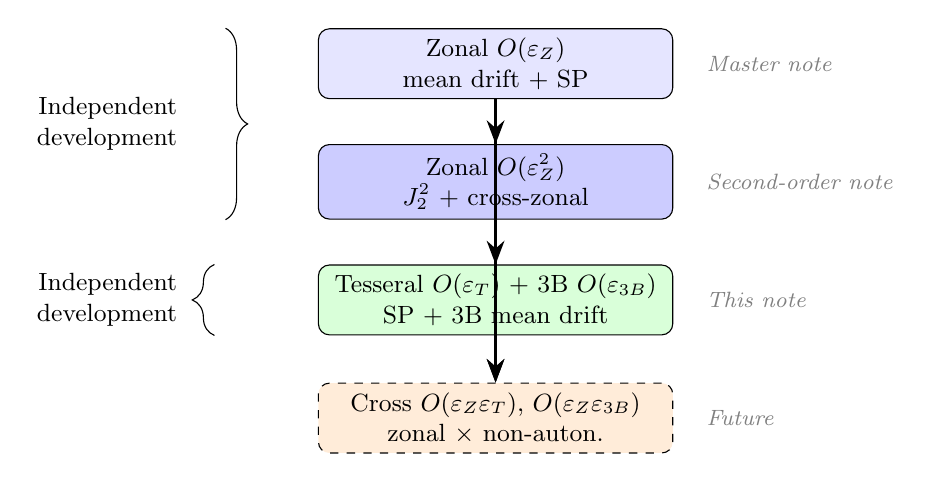
\begin{tikzpicture}[
    box/.style={draw, rounded corners, minimum width=4.5cm,
                minimum height=0.8cm, align=center, font=\small},
    arrow/.style={-{Stealth[length=3mm]}, thick},
    label/.style={font=\footnotesize\itshape, text=gray}
]

% Layer 1: Zonal baseline
\node[box, fill=blue!10] (z1) at (0, 0)
    {Zonal $O(\eps_Z)$\\mean drift + SP};
\node[label, right=0.3cm of z1] {Master note};

% Layer 2: Second-order zonal
\node[box, fill=blue!20] (z2) at (0, -1.5)
    {Zonal $O(\eps_Z^2)$\\$J_2^2$ + cross-zonal};
\node[label, right=0.3cm of z2] {Second-order note};

% Layer 3: Tesseral + 3B
\node[box, fill=green!15] (t1) at (0, -3.0)
    {Tesseral $O(\eps_T)$ + 3B $O(\eps_{3B})$\\SP + 3B mean drift};
\node[label, right=0.3cm of t1] {This note};

% Layer 4: Cross terms
\node[box, fill=orange!15, dashed] (cross) at (0, -4.5)
    {Cross $O(\eps_Z\eps_T)$, $O(\eps_Z\eps_{3B})$\\zonal $\times$ non-auton.};
\node[label, right=0.3cm of cross] {Future};

% Arrows
\draw[arrow] (z1) -- (z2);
\draw[arrow] (z1) -- (t1);
\draw[arrow] (z2) -- (cross);
\draw[arrow] (t1) -- (cross);

% Annotations
\draw[decorate, decoration={brace, amplitude=8pt, raise=2pt}]
    ([xshift=-3.5cm]z1.north) -- ([xshift=-3.5cm]z2.south)
    node[midway, left=12pt, font=\small, align=right]
    {Independent\\development};

\draw[decorate, decoration={brace, amplitude=8pt, raise=2pt, mirror}]
    ([xshift=-3.5cm]t1.north) -- ([xshift=-3.5cm]t1.south)
    node[midway, left=12pt, font=\small, align=right]
    {Independent\\development};

\end{tikzpicture}
\end{center}


%======================================================================
\section{Symbolic Complexity Estimates}
\label{sec:complexity}
%======================================================================

\subsection{Tesseral cost scaling}

For a tesseral harmonic of degree $n$ and order $m$:
\begin{itemize}
\item The surface harmonic $Y_n^{mc}$ is a polynomial of degree $n$ in
$(\hat x, \hat y, \hat z)$, contributing $O(n^2)$ monomials.
\item Each direction cosine has Laurent polynomial support of $O(1)$ in
$F$ (the expressions for $\hat x(F)$, $\hat y(F)$, $\hat z(F)$ have
fixed structure from the equinoctial rotation).
\item The total Laurent polynomial degree in $F$ grows as $O(n)$
(same as for zonals).
\item The number of $w$-harmonics is $O(n)$ (vs.\ $O(n)$ for zonals).
\item The additional $(\bar\Omega - \theta_G)$-harmonic content is
determined by $m$: each $(n,m)$ contributes harmonics at order exactly $m$
in $(\bar\Omega - \theta_G)$.
\end{itemize}

\begin{table}[ht]
\centering
\caption{Estimated symbolic computation scaling for tesseral harmonics,
compared to the known zonal costs.}
\label{tab:tesseral_cost}
\small
\begin{tabular}{@{}lccc@{}}
\toprule
Harmonic & Laurent terms & $\omega$-harmonics & Estimated time \\
\midrule
$J_2$ (zonal) & 14--21 & 1 & seconds \\
$C_{2,2}/S_{2,2}$ & $\sim$20--30 & 3 & $\sim$1 min \\
$C_{3,1}/S_{3,1}$ & $\sim$30--40 & 4 & $\sim$5 min \\
$C_{3,3}/S_{3,3}$ & $\sim$30--40 & 4 & $\sim$5 min \\
$C_{4,4}/S_{4,4}$ & $\sim$50--70 & 5 & $\sim$30 min \\
\midrule
$4 \times 4$ total & --- & --- & $\sim$2--4 hours \\
\bottomrule
\end{tabular}
\end{table}

These estimates are rough and based on extrapolation from the known zonal
scaling. The actual cost will depend on the complexity of the rational
coefficients after GCD simplification.

\subsection{Third-body cost scaling}

The third-body Legendre expansion at order $N_{3B}$:
\begin{itemize}
\item $N_{3B} = 2$: $P_2(\cos S)$ involves quadratic terms in the
direction cosines. Laurent polynomial degree comparable to $J_2$--$J_3$.
Estimated precomputation: minutes.
\item $N_{3B} = 3$: $P_3(\cos S)$ involves cubic terms. Laurent degree
comparable to $J_4$--$J_5$. Estimated: tens of minutes.
\end{itemize}

For most applications, $N_{3B} = 2$ suffices for the Moon (whose parallax
$a/r_{\text{Moon}} \sim 0.02$ for LEO) and $N_{3B} = 2$ for the Sun
(parallax $\sim 10^{-5}$).


%======================================================================
\section{Extensions and Alternatives}
\label{sec:extensions}
%======================================================================

\subsection{Resonance-aware extension}
\label{sec:resonance}

The theory as presented (Sections~\ref{sec:tesseral}--\ref{sec:operational})
is restricted to non-resonant orbits, where the tesseral mean drift vanishes
at first order. For orbits near a tesseral resonance
\begin{equation}
j\, n_0 \approx m\, \omega_E,
\qquad j, m \in \mathbb Z,
\end{equation}
(e.g., GEO at $j = m = 1$, GPS at $j = 2, m = 1$), the
near-resonant tesseral harmonics produce a non-vanishing mean drift and
the averaging breaks down for those specific harmonics.

\paragraph{Hybrid resonance approach.}
The natural extension is a hybrid method (Lara 2018, 2021):
\begin{enumerate}
\item Identify the near-resonant arguments
$\sigma_k = j_k \bar\lambda - m_k \theta_G + \ldots$ for the given orbit.
\item Promote each $\sigma_k$ to a slow variable with its own equation of
motion (pendulum-like resonance dynamics).
\item Average over the remaining (non-resonant) fast combinations as usual.
\item The resonant arguments contribute long-period oscillations
(libration) in the mean elements.
\end{enumerate}

This approach is compatible with the present framework:
\begin{itemize}
\item The non-resonant tesseral harmonics are handled exactly as in
Section~\ref{sec:tesseral} (short-period only).
\item The resonant harmonics are retained in the mean ODE, adding one or
more slow angles to the state vector.
\item The residue decomposition still applies to the non-resonant
short-period corrections.
\end{itemize}

The main implementation complexity is the orbit-dependent resonance
identification at initialization and the variable-dimension mean state.
This is deferred to a future extension, as it targets a narrower set of
applications (GEO station-keeping, navigation constellation management).

\subsection{Double-averaging (Kaula approach)}

An alternative to the single-averaging approach is the classical
double-averaging of Kaula (1966):
\begin{enumerate}
\item First average over the orbital fast angle (removing short-period terms).
\item Second average over the tesseral fast combination (removing
``medium-period'' tesseral oscillations at the sidereal-day timescale).
\end{enumerate}

The doubly-averaged system is autonomous and retains only the truly secular
and long-period components.

\paragraph{Trade-offs vs.\ single-averaging.}
\begin{center}
\begin{tabular}{lcc}
\toprule
Property & Single-averaging & Double-averaging \\
\midrule
Mean system & Non-autonomous & Autonomous \\
SP corrections & One layer & Two layers \\
Accuracy & Higher (one less avg.\ approx.) & Lower \\
Resonance handling & Deferred & Same difficulty \\
Third-body & Same framework & Requires $\ge 3$ frequencies \\
Generalizability & Any non-auton.\ source & Periodic sources only \\
\bottomrule
\end{tabular}
\end{center}

The single-averaging approach (Option~A) was chosen because it generalizes
naturally to \emph{any} non-autonomous perturbation (including
quasi-periodic third-body motion), whereas double-averaging requires each
additional frequency to be periodic with a known period.

\subsection{Extended phase space}

The non-autonomous mean ODE can be made formally autonomous by promoting
$\theta_G$ to a state variable with $\dot\theta_G = \omega_E$. This is
mathematically isomorphic to the non-autonomous formulation but may have
advantages for:
\begin{itemize}
\item Lie-transform analysis at higher order;
\item variational equations (STM) of the mean system;
\item Hamiltonian or symplectic structure preservation.
\end{itemize}

This option is noted but not pursued in the initial implementation.

\subsection{Solar radiation pressure}

SRP is structurally identical to third-body perturbation from the
perspective of the averaging framework:
\begin{itemize}
\item Non-autonomous (depends on Sun direction).
\item Conservative (in the simplest cannonball model).
\item The SRP acceleration is $\bm P_{\mathrm{SRP}} \propto
-\hat{\bm r}_\odot / r_\odot^2$, which is a constant vector during
the orbital average (frozen Sun direction).
\item The averaged SRP force produces both a mean drift (secular) and
short-period corrections.
\end{itemize}

The SRP extension would follow the same Phase~T3--T4 implementation path
as third-body, with the SRP acceleration replacing the third-body
acceleration. The $F$-variable structure is the same (SRP forcing is
linear in the direction cosines, hence a low-degree Laurent polynomial
in $F$).

\subsection{Time-angle correction for second-order tesseral theory}

As discussed in the compatibility analysis
(Section~\ref{sec:combined}), the frozen-$\theta_G$ approximation is
valid at first order and for the $O(\eps_Z \eps_T)$ cross terms, but
would break at $O(\eps_T^2)$ (where the freezing error is comparable
to the terms being captured). Since $\eps_T^2 \sim 10^{-12}$, this is
negligible in practice. However, for completeness:

A rigorous second-order tesseral theory would require replacing the
frozen-parameter orbital average with a ``corrected single-average'' that
accounts for the advance of $\theta_G$ during one revolution:
\begin{equation}
\theta_G(t(K)) = \theta_G(t_0) + \omega_E \cdot \frac{M(K)}{n_0},
\end{equation}
where $M(K) = K - g\sin K$ is the mean anomaly. The factor
$e^{-im\omega_E M(K)/n_0}$ is transcendental in $K$ (not a Laurent
polynomial in $F$), which would break the rational-in-$F$ structure.

Two mitigation paths exist:
\begin{enumerate}
\item Expand the time correction as a Fourier-Bessel series in $K$,
converting the transcendental factor to a truncated Laurent series.
\item Adopt a Fourier/Hansen approach for the tesseral second-order terms
only, computing the corrections as Fourier series in the mean longitude
$\lambda$ (the natural variable for time-dependent averaging) rather
than through the $F$-variable residue decomposition.
\end{enumerate}

Neither path is needed for the present first-order extension.


%======================================================================
\section{Publication Strategy}
\label{sec:publication}
%======================================================================

The work decomposes into four independent publications, ordered by
decreasing readiness:

\begin{enumerate}
\item \textbf{Paper 1} (master note): First-order averaged GEqOE theory
for autonomous zonal harmonics. \emph{Status: complete, ready for
submission.}

\item \textbf{Paper 2} (second-order note): Second-order near-identity
averaging for GEqOE under zonals. Independent of the non-autonomous
extension. \emph{Status: framework sketched, implementation pending.}

\item \textbf{Paper 3} (this note): First-order non-autonomous extension
to tesseral harmonics and third-body. Builds on Paper~1; independent of
Paper~2. Demonstrates that the residue decomposition generalizes beyond
the autonomous case. \emph{Status: plan documented, implementation
pending.}

\item \textbf{Paper 4} (future): Combined second-order zonal + first-order
non-autonomous theory. Merges Papers~2 and~3 and adds the cross-coupling
layer $O(\eps_Z \eps_T)$, $O(\eps_Z \eps_{3B})$. \emph{Status: design
specified in this note (Section~\ref{sec:combined}), implementation
requires Papers~2 and~3.}
\end{enumerate}

The key novelty claim for Paper~3 is the demonstration that the
$F$-variable residue decomposition method---originally developed for the
autonomous zonal problem---generalizes constructively to non-autonomous
perturbations (tesseral and third-body), producing closed-form
short-period corrections in a non-canonical element set (GEqOE) where
the existing literature relies on either numerical quadrature
(DSST tradition) or canonical Lie transforms (Deprit/Lara tradition).


%======================================================================
\section{Summary}
\label{sec:summary}
%======================================================================

\begin{enumerate}
\item The GEqOE averaged theory extends to non-autonomous perturbations
(tesseral harmonics, lunisolar third-body) via \textbf{single-averaging
over the orbital fast angle $K$ with frozen non-autonomous parameters}.

\item The tesseral and third-body forcing functions are \textbf{rational
functions of $F$} with the same fixed pole structure
$(F+q)^2(1+qF)^2$ as the zonal forcing. The direct residue decomposition
applies without modification.

\item The mean-element ODE becomes \textbf{non-autonomous but smooth and
slowly varying}. For non-resonant orbits, the tesseral mean drift vanishes
at first order; third-body contributes a nonzero mean drift parameterized
by the ephemeris direction.

\item The extension is \textbf{modular}: zonal, tesseral, and third-body
contributions are additive in both the mean drift and the short-period
corrections.

\item The extension is \textbf{compatible with the second-order zonal
theory}: the two developments proceed independently and merge into a
combined $O(\eps_Z^2) + O(\eps_T) + O(\eps_{3B})$ theory. The cross
terms $O(\eps_Z \eps_T)$ and $O(\eps_Z \eps_{3B})$ remain within the
rational-in-$F$ framework and can be computed by the same residue
algorithm.

\item \textbf{Resonance handling} (GEO, GPS) is architecturally compatible
as a future add-on layer but is deferred from the initial implementation.
\end{enumerate}


\begin{thebibliography}{99}

\bibitem{bau2021}
Ba\`u, G., Hernando-Ayuso, J., Bombardelli, C. (2021).
A generalization of the equinoctial orbital elements.
\textit{Celestial Mechanics and Dynamical Astronomy}, 133, 50.

\bibitem{brouwer1959}
Brouwer, D. (1959).
Solution of the problem of artificial satellite theory without drag.
\textit{The Astronomical Journal}, 64, 378--396.

\bibitem{kaula1966}
Kaula, W.\,M. (1966).
\textit{Theory of Satellite Geodesy}.
Blaisdell, Waltham, MA.

\bibitem{deprit1969}
Deprit, A. (1969).
Canonical transformations depending on a small parameter.
\textit{Celestial Mechanics}, 1, 12--30.

\bibitem{cefola1972}
Cefola, P.\,J. (1972).
Equinoctial orbit elements---application to artificial satellite orbits.
AIAA Paper 72-937.

\bibitem{danielson1995}
Danielson, D.\,A., Neta, B., Early, L.\,W. (1995).
Semianalytic satellite theory.
Naval Postgraduate School Technical Report NPS-MA-95-002.

\bibitem{lara2018}
Lara, M. (2018).
On the non-integrability of the tesseral problem in satellite theory.
\textit{Celestial Mechanics and Dynamical Astronomy}, 130, 69.

\bibitem{lara2021}
Lara, M. (2021).
Brouwer's satellite solution redux.
\textit{Celestial Mechanics and Dynamical Astronomy}, 133, 47.

\bibitem{metris1995}
M\'etris, G., Exertier, P. (1995).
Semi-analytical theory of the mean orbital motion.
\textit{Astronomy and Astrophysics}, 294, 278--286.

\bibitem{sanjuan2022}
San-Juan, J.\,F., L\'opez, R., Cefola, P.\,J. (2022).
A second-order closed-form $J_2$ model for the Draper
Semi-Analytical Satellite Theory.
\textit{The Journal of the Astronautical Sciences}, 69, 1292--1318.

\bibitem{mahajan2019}
Mahajan, B., Alfriend, K.\,T. (2019).
Analytic orbit theory with any arbitrary spherical harmonic as the
dominant perturbation.
\textit{Celestial Mechanics and Dynamical Astronomy}, 131, 45.

\bibitem{biscani2021}
Biscani, F., Izzo, D. (2021).
Revisiting high-order Taylor methods for astrodynamics and celestial
mechanics.
\textit{Monthly Notices of the Royal Astronomical Society}, 504(2),
2614--2628.

\end{thebibliography}

\end{document}
